% Options for packages loaded elsewhere
\PassOptionsToPackage{unicode}{hyperref}
\PassOptionsToPackage{hyphens}{url}
%
\documentclass[
  12pt,
]{article}
\usepackage{lmodern}
\usepackage{amssymb,amsmath}
\usepackage{ifxetex,ifluatex}
\ifnum 0\ifxetex 1\fi\ifluatex 1\fi=0 % if pdftex
  \usepackage[T1]{fontenc}
  \usepackage[utf8]{inputenc}
  \usepackage{textcomp} % provide euro and other symbols
\else % if luatex or xetex
  \usepackage{unicode-math}
  \defaultfontfeatures{Scale=MatchLowercase}
  \defaultfontfeatures[\rmfamily]{Ligatures=TeX,Scale=1}
\fi
% Use upquote if available, for straight quotes in verbatim environments
\IfFileExists{upquote.sty}{\usepackage{upquote}}{}
\IfFileExists{microtype.sty}{% use microtype if available
  \usepackage[]{microtype}
  \UseMicrotypeSet[protrusion]{basicmath} % disable protrusion for tt fonts
}{}
\makeatletter
\@ifundefined{KOMAClassName}{% if non-KOMA class
  \IfFileExists{parskip.sty}{%
    \usepackage{parskip}
  }{% else
    \setlength{\parindent}{0pt}
    \setlength{\parskip}{6pt plus 2pt minus 1pt}}
}{% if KOMA class
  \KOMAoptions{parskip=half}}
\makeatother
\usepackage{xcolor}
\IfFileExists{xurl.sty}{\usepackage{xurl}}{} % add URL line breaks if available
\IfFileExists{bookmark.sty}{\usepackage{bookmark}}{\usepackage{hyperref}}
\hypersetup{
  pdftitle={Hurricane Michael and Floridian Turnout},
  pdfauthor={Kevin Morris; Peter Miller},
  hidelinks,
  pdfcreator={LaTeX via pandoc}}
\urlstyle{same} % disable monospaced font for URLs
\usepackage[margin=1in]{geometry}
\usepackage{longtable,booktabs}
% Correct order of tables after \paragraph or \subparagraph
\usepackage{etoolbox}
\makeatletter
\patchcmd\longtable{\par}{\if@noskipsec\mbox{}\fi\par}{}{}
\makeatother
% Allow footnotes in longtable head/foot
\IfFileExists{footnotehyper.sty}{\usepackage{footnotehyper}}{\usepackage{footnote}}
\makesavenoteenv{longtable}
\usepackage{graphicx}
\makeatletter
\def\maxwidth{\ifdim\Gin@nat@width>\linewidth\linewidth\else\Gin@nat@width\fi}
\def\maxheight{\ifdim\Gin@nat@height>\textheight\textheight\else\Gin@nat@height\fi}
\makeatother
% Scale images if necessary, so that they will not overflow the page
% margins by default, and it is still possible to overwrite the defaults
% using explicit options in \includegraphics[width, height, ...]{}
\setkeys{Gin}{width=\maxwidth,height=\maxheight,keepaspectratio}
% Set default figure placement to htbp
\makeatletter
\def\fps@figure{htbp}
\makeatother
\setlength{\emergencystretch}{3em} % prevent overfull lines
\providecommand{\tightlist}{%
  \setlength{\itemsep}{0pt}\setlength{\parskip}{0pt}}
\setcounter{secnumdepth}{5}
\usepackage{rotating}
\usepackage{setspace}
\newcommand{\beginsupplement}{\setcounter{table}{0}  \renewcommand{\thetable}{A\arabic{table}} \setcounter{figure}{0} \renewcommand{\thefigure}{A\arabic{figure}}}
\usepackage{booktabs}
\usepackage{longtable}
\usepackage{array}
\usepackage{multirow}
\usepackage{wrapfig}
\usepackage{float}
\usepackage{colortbl}
\usepackage{pdflscape}
\usepackage{tabu}
\usepackage{threeparttable}
\usepackage{threeparttablex}
\usepackage[normalem]{ulem}
\usepackage{makecell}
\usepackage{xcolor}
\newlength{\cslhangindent}
\setlength{\cslhangindent}{1.5em}
\newenvironment{cslreferences}%
  {\setlength{\parindent}{0pt}%
  \everypar{\setlength{\hangindent}{\cslhangindent}}\ignorespaces}%
  {\par}

\title{Hurricane Michael and Floridian Turnout\thanks{The authors thanks Many People for their comments on this project. All errors are our responsibility.}}
\author{Kevin Morris\footnote{Researcher, Brennan Center for Justice at NYU School of Law, 120 Broadway Ste 1750, New York, NY 10271 (\href{mailto:kevin.morris@nyu.edu}{\nolinkurl{kevin.morris@nyu.edu}})} \and Peter Miller\footnote{Researcher, Brennan Center for Justice at NYU School of Law, 120 Broadway Ste 1750, New York, NY 10271 (\href{mailto:peter.miller@nyu.edu}{\nolinkurl{peter.miller@nyu.edu}})}}
\date{March 23, 2020}

\begin{document}
\maketitle
\begin{abstract}
This is an abstract.
\end{abstract}

\pagenumbering{gobble}
\pagebreak

\pagenumbering{arabic}
\doublespacing

\hypertarget{research-design-and-expectations}{%
\section*{Research Design and Expectations}\label{research-design-and-expectations}}
\addcontentsline{toc}{section}{Research Design and Expectations}

Based on prior research, we expect that turnout was substantially depressed in the treated counties in 2018. This depressed turnout, however, was likely caused by both individual- and administrative-level mechanisms.

\hypertarget{individual-level-effects}{%
\subsection*{Individual-Level Effects}\label{individual-level-effects}}
\addcontentsline{toc}{subsection}{Individual-Level Effects}

We know that Hurricane Michael caused substantial destruction; as discussed in the introduction to this paper, residents lost their lives, flooding was widespread, and the hurricane caused billions of dollars of property damage. Would-be voters were now faced with myriad disruptions to their daily lives; it is likely that the direct effects of the weather, therefore, reduced turnout substantially. As professor emeritus Robert Montjoy told NPR in the aftermath of the storm, ``Whether casting a ballot becomes a higher priority than cleaning out the basement, visiting someone in the hospital, or all the other demands\ldots You certainly expect a lower turnout for those reasons'' (Parks \protect\hyperlink{ref-Parks2018}{2018}).

\hypertarget{administrative-effects}{%
\subsection*{Administrative Effects}\label{administrative-effects}}
\addcontentsline{toc}{subsection}{Administrative Effects}

The hurricane also caused problems for county election administrators, as the reporting around the Governor's executive order makes clear.\footnote{Executive Order 18-283 can be found here: \url{https://www.flgov.com/wp-content/uploads/2018/10/SLT-BIZHUB18101809500.pdf}. In the event that this link no longer works, it is on file with the authors.} Polling places were destroyed; some mail voters were residing in locations other than their registered addresses; would-be poll workers were unavailable. These factors could have increased the costs of voting even for residents who were not directly impacted by the hurricane, and increased the costs of voting even more for individuals who were directly impacted. Absent mitigation, the administrative effects of Hurricane Michael likely would have decreased turnout above-and-beyond the individual effects of the storm.

Executive Order 18-283 sought to offset the administrative barriers to voting by allowing county election administrators to flexibly respond to the damage wrought by the storm. Specifically, Executive Order 18-283 allowed administrators to add early voting locations; begin early voting 15 days before the general election, and continue until the day of the election; to accept vote-by-mail requests to addresses other than a voter's registered address; to send vote-by-mail ballots by forwardable mail; to deliver vote-by-mail ballots to electors or electors' immediate family members on election day without an affidavit; to relocate or consolidate polling places; and required poll watchers to be registered by the second Friday before the general election.

This paper sets out to answer two questions: what was the total depressive effect of the hurricane? And did Executive Order 18-283 effectively offset the depressive administrative effects?

\hypertarget{estimating-the-net-effects-of-the-hurricane}{%
\subsection*{Estimating the Net Effects of the Hurricane}\label{estimating-the-net-effects-of-the-hurricane}}
\addcontentsline{toc}{subsection}{Estimating the Net Effects of the Hurricane}

We begin by testing the net effect of each of these treatments on individual-level turnout. Our central identification strategy involves the use of difference-in-differences models. By comparing historical and 2018 turnout for voters in the counties hit by the storm to historical and 2018 turnout of voters elsewhere in the state, we can estimate the effect of the storm on turnout. To ensure a high-quality difference-in-differences specification, we do not include all untreated voters in our control group; rather, we match each treated voter with five untreated voters along a battery of individual- and neighborhood-level characteristics. Untreated voters who do not serve as matches are excluded from our models. Although it may seem counterintuitive to exclude data from our models, this matching procedure substantially improves the parallel trends assumptions necessary for a rigorous difference-in-differences analysis.

This design allows us to test our first hypothesis:

\textbf{Hypothesis 1:} Turnout in the eight treated counties was lower in 2018 due to the combined effects of the hurricane, county-level responses, and the executive order.

\hypertarget{testing-adminstrative-effects}{%
\subsection*{Testing Adminstrative Effects}\label{testing-adminstrative-effects}}
\addcontentsline{toc}{subsection}{Testing Adminstrative Effects}

To estimate the administrative effect on turnout, we must control for the individual-level effects of the storm. To do so, we leverage the somewhat arbitrary borders of counties in the Florida Panhandle. There is no reason to believe that the effects of a hurricane would change dramatically along county borders. We assume, therefore, that voters who lived nearby one another, but on either side of a county border, faced the same weather issues during the 2018 election. Any difference in turnout observed between groups that live just over a county border from one another, therefore, can be attributed to the administration of the election in their respective county.

To disaggregate the individual and administrative effects of Hurricane Michael, we employ a double-matched triple-differences (or difference-in-difference-in-differences) specification.

We begin by constructing our set of treated voters. These treated voters include all registered voters who live in a treated county and within two miles of a bordering, untreated county. Each treated voter is then each matched to one voter who lives in an untreated county, but within two miles of a treated county. As discussed above, we assume that the only difference between each member of each pair is the administrative context in which they lived because they lived in close geographic proximity to one another. These matches form our set of ``primary control voters.''

Each treated and primary control voter is subsequently matched to five voters elsewhere in the state --- that is to say, voters who are neither in the treated counties nor in the counties directly surrounding the treated counties. This exercise is the second match, and the matches are our ``secondary control voters.''

At this point, we have four distinct groups of voters: treated voters; primary control voters; secondary control voters who serve as controls for the treated voters; and secondary control voters who serve as controls for the primary control voters. While the treated, primary control, and full set of secondary control voters are mutually exclusive, secondary control voters are allowed to serve as controls for each of the other two groups. Indeed, because the primary control voters have been selected to resemble the treated voters, overlaps among these groups is highly likely.

Having constructed our pool of voters, we run a triple-differences model. This triple-differences model is, in effect, two simultaneous difference-in-differences models. The model begins\footnote{In reality, the model estimates each of the following steps simultaneously; for narrative purposes, we describe the effects of the model in a sequential fashion.} by estimating whether 2018 was associated with depressed turnout for our primary control voters vis-à-vis their (matched, secondary) controls and their own vote history. Because these primary control voters lived in counties not covered by the executive order, we assume that they faced no administrative effects from the storm; any observed difference in turnout, therefore, can be attributed to the individual-level effects of the storm.

The model then estimates a second difference-in-differences model, asking whether 2018 was associated with depressed turnout for treated voters vis-à-vis their (matched, secondary) controls and their own vote history. This model estimates the net individual- and administrative-level effects faced by treated voters in 2018.

The model finally estimates the difference in the treatment associated with 2018 for the treated and primary control voters. Because the only difference between treated and primary control voters is the administrative district in which they lived, this estimated difference is interpreted as the adminstrative effect on turnout in the treated counties.

The double-matched triple-differences model allows us to test our second hypothesis:

\textbf{Hypothesis 2:} After controlling for weather, we expect that turnout in the treated counties was slightly lower than in untreated counties. We expect that Executive Order 18-283 was largely, but not entirely, successful at offsetting the depressive administrative effects of Hurricane Michael.

\hypertarget{results}{%
\section*{Results}\label{results}}
\addcontentsline{toc}{section}{Results}

\hypertarget{overall-turnout-effects}{%
\subsection*{Overall Turnout Effects}\label{overall-turnout-effects}}
\addcontentsline{toc}{subsection}{Overall Turnout Effects}

We begin by matching each registered voter in the eight treated counties to five untreated voters elsewhere in the state using a genetic matching algorithm (Sekhon \protect\hyperlink{ref-Sekhon2011}{2011}).\footnote{Due to computing constraints, the matching weights were constructed using a one percent random sample stratified by treatment status.} The individual-level characteristics come directly from the registered voter file. The two neighborhood-level characteristics included --- median income and share of the population with some collegiate education --- are estimated at the block group level, and come from the ACS 5-year estimates ending with 2018. Ties are not broken, which means that some treated voters are assigned more than five control voters; the weights used in the regressions below are adjusted accordingly.

Although the treated counties were the at the center of the storm, nearby counties might have also been negatively impacted by the storm. Therefore, voters who live in the counties that border the treated counties are excluded. These include Walton, Holmes, Wakulla, and Leon Counties.

Table \ref{tab:full-bal} demonstrates the results of this matching procedure. As Table \ref{tab:full-bal} makes clear, voters in the affected counties were considerably more likely to be white and identify as Republicans, and live in lower-income neighborhoods, than voters in the rest of the state. The post-match control group, however, looks substantially similar to the treated voters.

\begin{singlespace}
\begin{table}[H]

\caption{\label{tab:balance-tab-full}\label{tab:full-bal} Balance Table for Statewide Matching}
\centering
\resizebox{\linewidth}{!}{
\begin{tabular}[t]{lllllrrrr}
\toprule
\multicolumn{1}{c}{ } & \multicolumn{2}{c}{Means: Unmatched Data} & \multicolumn{2}{c}{Means: Matched Data} & \multicolumn{4}{c}{Percent Improvement} \\
\cmidrule(l{3pt}r{3pt}){2-3} \cmidrule(l{3pt}r{3pt}){4-5} \cmidrule(l{3pt}r{3pt}){6-9}
 & Treated & Control & Treated & Control & Mean Diff & eQQ Med & eQQ Mean & eQQ Max\\
\midrule
\%White & 77.0\% & 62.0\% & 77.0\% & 77.0\% & 100.00 & 100.00 & 100.00 & 100.00\\
\% Black & 17.0\% & 13.0\% & 17.0\% & 17.0\% & 100.00 & 100.00 & 100.00 & 100.00\\
\% Latino & 2.0\% & 17.0\% & 2.0\% & 2.0\% & 100.00 & 100.00 & 100.00 & 100.00\\
\% Asian & 1.0\% & 2.0\% & 1.0\% & 1.0\% & 100.00 & 100.00 & 100.00 & 100.00\\
\% Female & 53.0\% & 52.0\% & 53.0\% & 53.0\% & 100.00 & 100.00 & 100.00 & 100.00\\
\% Male & 46.0\% & 45.0\% & 46.0\% & 46.0\% & 100.00 & 100.00 & 100.00 & 100.00\\
Age & 52.23 & 52.49 & 52.23 & 52.23 & 97.76 & 94.17 & 94.71 & 94.05\\
\% Democrat & 39.0\% & 37.0\% & 39.0\% & 39.0\% & 100.00 & 100.00 & 100.00 & 100.00\\
\% Republican & 44.0\% & 35.0\% & 44.0\% & 44.0\% & 100.00 & 100.00 & 100.00 & 100.00\\
\% with Some College & 69.0\% & 75.0\% & 69.0\% & 69.0\% & 99.79 & 99.29 & 98.38 & 89.71\\
Median Income & \$50,643 & \$62,941 & \$50,643 & \$50,659 & 99.87 & 97.55 & 96.13 & 84.03\\
\bottomrule
\end{tabular}}
\end{table}
\end{singlespace}

After matching the individual voters, we can construct historical turnout estimates for the treated and control voters. Figure \ref{fig:full-to} plots the turnout in the past few elections for our treated and control voters. As Figure \ref{fig:full-to} makes clear, treated voters consistently turned out at higher rates than control voters from 2010 -- 2016. In 2018 however --- the year when Hurricane Michael wreaked havoc on voters in the treatment group --- this relationship was inverted as turnout among treated voters plummeted from its 2016 level. Although turnout among all voters was higher in 2018 than in 2014, turnout rose by substantially less for the treated voters.

\begin{figure}[H]

{\centering 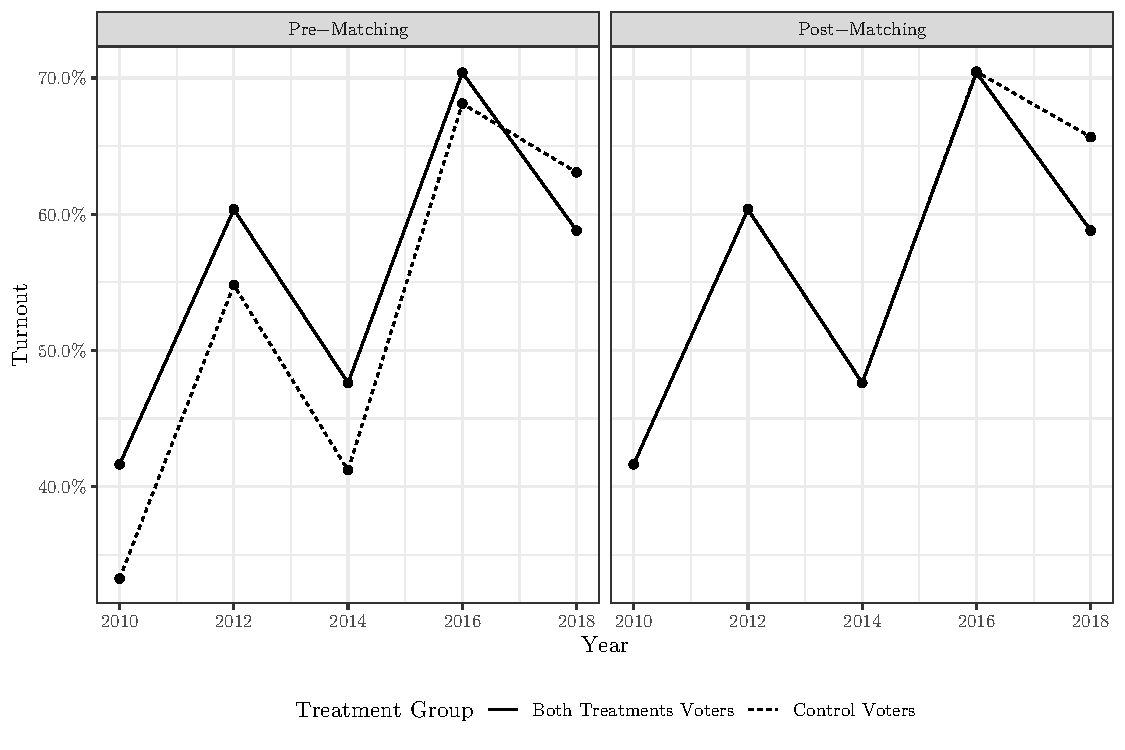
\includegraphics{hurricane_michael_files/figure-latex/full-to-chunk-1} 

}

\caption{\label{fig:full-to}General Election Turnout for Treated and Control Voters, 2010 -- 2018}\label{fig:full-to-chunk}
\end{figure}

Table \ref{tab:full-dind} formalizes Figure \ref{fig:full-to} into a differences-in-differences regression specification. We employ an ordinary least squares specification.\footnote{Although the dependent variable here is binary --- it takes the value 0 if a voter does not participate, and 1 if she does --- the coefficients produced by logistic regressions in the difference-in-differences context are largely uninterpretable. We thus use a linear specification here. When the models are estimated using a logistic specification, the treatment effect is consistent.} The dependent variable takes the value 1 if a voter cast a ballot in a given year, and 0 if she did not. Model 1 includes only three variables in addition to the constant. \emph{Treated} measures the gap between treated and control voters in the 2010 -- 2016 period. \emph{2018} measures the increase in turnout observed among control voters in 2018, while \emph{Treated × 2018} measures whether turnout in 2018 departed further or less from the baseline for the treated voters than the control voters. Model 2 includes the same variables, but also includes the characteristics on which the voters were matched. Model 3, finally, also includes measures for congressional district competitiveness. Because this variable is ``downstream'' of treatment --- that is to say, the effect of the hurricane could have impacted the competitiveness of certain races --- it is not included in the first two models. It should be noted that each of the treated voters lived in uncontested congressional districts. Robust standard errors are clustered at the level of the match (Abadie and Spiess \protect\hyperlink{ref-Abadie2019}{2019}).

\begin{singlespace}
\input{"../temp/dind_full.tex"}
\end{singlespace}

The coefficient on \emph{Treated × 2018} in Table \ref{tab:full-dind} indicates that Hurricane Michael had a substantial depressive effect in 2018 among the treated voters. Each model estimates that the overall effect --- including individual and administrative effects --- was -8.4 percentage points. Multiplied across the nearly 200 thousand registered voters in the treated counties indicates that some 16 thousand ballots went uncast due to the hurricane --- a major effect in a year when a statewide senate race was decided by 10,033 votes.

\hypertarget{identifying-adminstrative-effects}{%
\subsection*{Identifying Adminstrative Effects}\label{identifying-adminstrative-effects}}
\addcontentsline{toc}{subsection}{Identifying Adminstrative Effects}

As discussed above, our primary strategy for isolating the administrative effects of the hurricane on turnout involves leveraging random assignment around county borders in the Florida panhandle in a double-matched triple-differences specification. This specification involves matching voters in treated counties to voters in neighboring, untreated counties. This allows us to control for weather effects, while letting the administrative context vary. Treated and these matched, ``primary control voters'' are then matched to voters elsewhere in the state, allowing us to test the overall effect of the storm on turnout. By comparing the treatment effect for the primary control voters to the treatment voters in a triple-differences framework, we can decompose the individual-level effects from the administrative effects of Hurricane Michael.

We begin by identifying all voters who lived within two miles of a county with a different treatment status. Figure \ref{fig:map} shows the map of counties in the region. The eight treated counties are drawn in a medium gray, and the untreated border counties are drawn in dark gray. All treated and control voters come from the light gray buffer, which extends for two miles on either side of the border between a treated and untreated county. There are not voters in Gulf, Calhoun, or Franklin Counties who live within two miles of an untreated county.

\begin{figure}[H]

{\centering 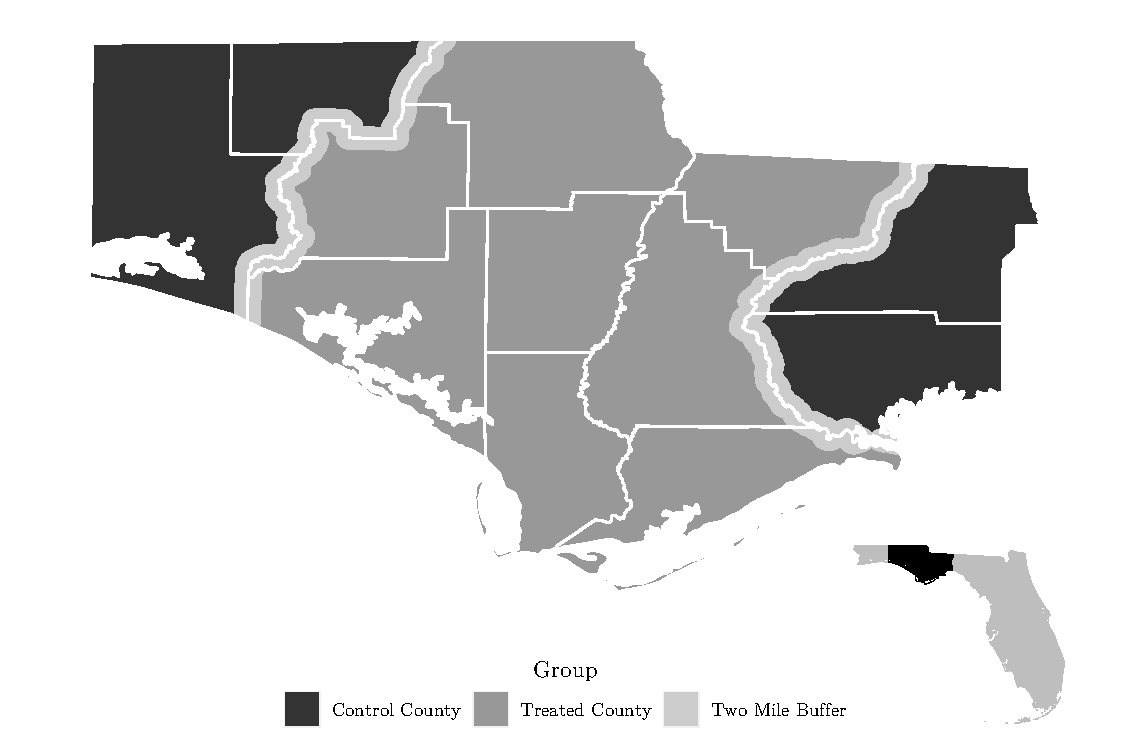
\includegraphics{hurricane_michael_files/figure-latex/map-chunk-1} 

}

\caption{\label{fig:map}Treated and Control Counties with Two Mile Buffer}\label{fig:map-chunk}
\end{figure}

Each voter inside the buffer in a treated county is matched with one voter in the buffer in an untreated county, once again using the genetic matching algorithm developed by Sekhon (\protect\hyperlink{ref-Sekhon2011}{2011}). These matches serve as our primary control voters. Ties are not broken, which means that some treated voters are assigned multiple primary control voters; the weights used in the regressions below are adjusted accordingly.

In some cases, voters on either side of the border are in different congressional districts. This would pose a problem if these races were contested thanks to the potentially mobilizing effects of house races, but the entire buffer falls in uncontested congressional districts. This means that treated and untreated voters are not facing differential mobilization from congressional races. As before, we match on individual- and neighborhood-level characteristics. Importantly, we match treated and untreated voters using their latitude and longitude to ensure that matches live in close proximity to one another. Table \ref{tab:balance-ll} presents the results of this matching exercise.

\begin{singlespace}
\begin{table}[H]

\caption{\label{tab:balance-tab-ll}\label{tab:balance-ll} Balance Table for Border Buffer Matching}
\centering
\resizebox{\linewidth}{!}{
\begin{tabular}[t]{lllllrrrr}
\toprule
\multicolumn{1}{c}{ } & \multicolumn{2}{c}{Means: Unmatched Data} & \multicolumn{2}{c}{Means: Matched Data} & \multicolumn{4}{c}{Percent Improvement} \\
\cmidrule(l{3pt}r{3pt}){2-3} \cmidrule(l{3pt}r{3pt}){4-5} \cmidrule(l{3pt}r{3pt}){6-9}
 & Treated & Control & Treated & Control & Mean Diff & eQQ Med & eQQ Mean & eQQ Max\\
\midrule
\%White & 74.9\% & 82.7\% & 74.9\% & 74.9\% & 100.00 & 100.00 & 100.00 & 100.00\\
\% Black & 20.7\% & 12.1\% & 20.7\% & 20.4\% & 96.51 & 96.63 & 96.63 & 96.63\\
\% Latino & 1.5\% & 1.6\% & 1.5\% & 1.3\% & -153.02 & -144.51 & -144.51 & -144.51\\
\% Asian & 0.4\% & 0.5\% & 0.4\% & 0.4\% & 100.00 & 100.00 & 100.00 & 100.00\\
\% Female & 53.4\% & 52.8\% & 53.4\% & 53.4\% & 98.07 & 98.13 & 98.13 & 98.13\\
\% Male & 45.4\% & 45.7\% & 45.4\% & 45.5\% & 76.18 & 76.98 & 76.98 & 76.98\\
Age & 52.536 & 51.612 & 52.536 & 52.446 & 90.26 & 72.06 & 70.58 & 60.06\\
\% Democrat & 44.2\% & 38.8\% & 44.2\% & 44.2\% & 100.00 & 100.00 & 100.00 & 100.00\\
\% Republican & 41.9\% & 45.0\% & 41.9\% & 41.9\% & 99.47 & 99.48 & 99.48 & 99.48\\
\% with Some College & 63.8\% & 66.7\% & 63.8\% & 65.0\% & 58.28 & 43.39 & 26.07 & -17.56\\
Median Income & \$47,598 & \$49,407 & \$47,598 & \$47,242 & 80.30 & -26.88 & -17.50 & 11.06\\
\bottomrule
\end{tabular}}
\end{table}
\end{singlespace}

The match procedure improves the balance between treated and primary control voters substantially for 10 of the 11 characteristics listed in Table \ref{tab:balance-ll}. The share Latino --- the only characteristic to go unimproved --- is below 2 percent for both groups and the difference is unlikely to cause any problems. Although latitudes and longitudes are not displayed in the table, the average treated voter lives just 8 miles from her primary control voter. This distance satisfies our assumption that treated and primary control voters faced the same weather effects from the hurricane. Figure \ref{fig:ll-to} makes clear that the parallel trends assumption is satisfied for post-matching treated and primary control voters.

\begin{figure}[H]

{\centering 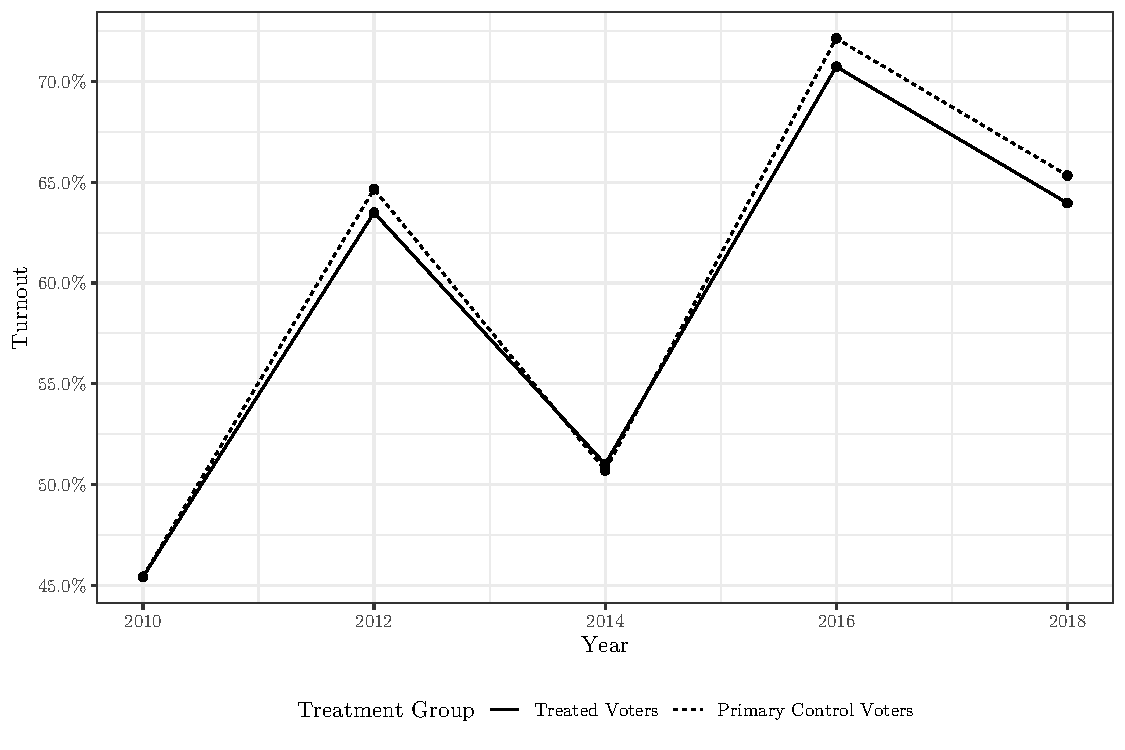
\includegraphics{hurricane_michael_files/figure-latex/ll-to-chunk-1} 

}

\caption{\label{fig:ll-to}General Election Turnout for Treated and Primary Control Voters, 2010 -- 2018}\label{fig:ll-to-chunk}
\end{figure}

Once our set of treated and primary control voters has been identified, each of these voters is matched with five other voters that lived in neither the treated nor the immediately surrounding counties. For ease of notation, the combined set of treated and primary control voters will henceforth be refered to as ``Panhandle voters,'' while ``treated'' voters will distinguish Panhandle voters in treated counties from Panhandle voters in other counties. The use of ``Panhandle'' is a slight misnomer: it excludes Escambia, Santa Rosa, and Okaloosa Counties which are certainly part of the Florida Panhandle, as well as Jefferson County and others to its east which are sometimes considered part of the panhandle. Nevertheless, we adopt this (hopefully inoffensive) shorthand for referring to the treated counties and their neighbors.

This matching procedure follows the same steps detailed in the Overall Turnout Effects section of this paper. Table \ref{tab:balance-secondary} presents the results of the secondary match. We improve along all characteristics.

\begin{singlespace}
\begin{table}[H]

\caption{\label{tab:balance-tab-ll2}\label{tab:balance-secondary} Balance Table for Secondary Match}
\centering
\resizebox{\linewidth}{!}{
\begin{tabular}[t]{lllllrrrr}
\toprule
\multicolumn{1}{c}{ } & \multicolumn{2}{c}{Means: Unmatched Data} & \multicolumn{2}{c}{Means: Matched Data} & \multicolumn{4}{c}{Percent Improvement} \\
\cmidrule(l{3pt}r{3pt}){2-3} \cmidrule(l{3pt}r{3pt}){4-5} \cmidrule(l{3pt}r{3pt}){6-9}
 & Treated & Control & Treated & Control & Mean Diff & eQQ Med & eQQ Mean & eQQ Max\\
\midrule
\%White & 74.9\% & 62.3\% & 74.9\% & 74.9\% & 100.00 & 100.00 & 100.00 & 100.00\\
\% Black & 19.7\% & 13.1\% & 19.7\% & 19.7\% & 100.00 & 100.00 & 100.00 & 100.00\\
\% Latino & 1.8\% & 17.4\% & 1.8\% & 1.8\% & 100.00 & 100.00 & 100.00 & 100.00\\
\% Asian & 0.5\% & 2.0\% & 0.5\% & 0.5\% & 100.00 & 100.00 & 100.00 & 100.00\\
\% Female & 53.0\% & 52.4\% & 53.0\% & 53.0\% & 100.00 & 100.00 & 100.00 & 100.00\\
\% Male & 45.6\% & 44.9\% & 45.6\% & 45.6\% & 100.00 & 100.00 & 100.00 & 100.00\\
Age & 52.403 & 52.489 & 52.403 & 52.398 & 93.30 & 90.74 & 88.85 & 80.02\\
\% Democrat & 43.6\% & 37.1\% & 43.6\% & 43.6\% & 100.00 & 100.00 & 100.00 & 100.00\\
\% Republican & 41.3\% & 35.0\% & 41.3\% & 41.3\% & 100.00 & 100.00 & 100.00 & 100.00\\
\% with Some College & 63.8\% & 75.1\% & 63.8\% & 63.8\% & 99.94 & 99.79 & 98.00 & 74.54\\
Median Income & \$47,154 & \$62,941 & \$47,154 & \$47,003 & 99.05 & 97.51 & 93.67 & 73.01\\
\bottomrule
\end{tabular}}
\end{table}
\end{singlespace}

Figure \ref{fig:second-parallel} demonstrates that the parallel trends assumption holds: turnout among the secondary controls tracks neatly with the turnout of the Panhandle voters prior to 2018. Although Figure \ref{fig:second-parallel} demonstrates that turnout among Panhandle voters was depressed in 2018, it does not allow us to distinguish between the individual and administrative effects.

\begin{figure}[H]

{\centering 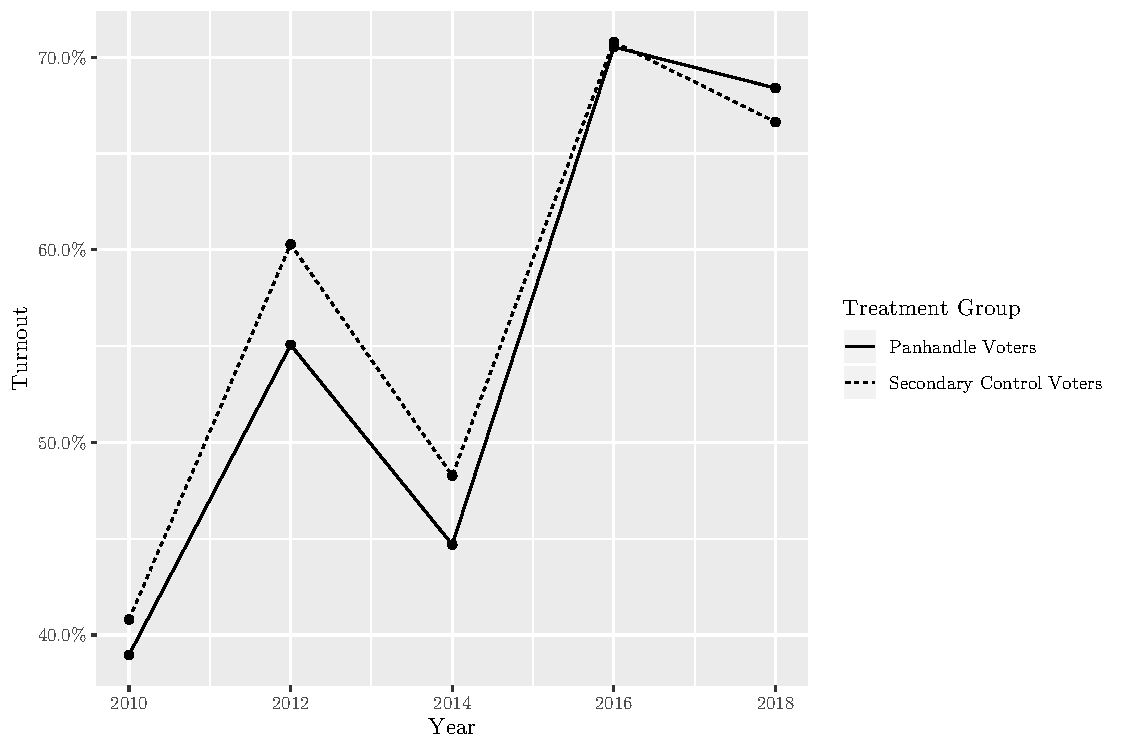
\includegraphics{hurricane_michael_files/figure-latex/second-parallel-chunk-1} 

}

\caption{\label{fig:second-parallel}General Election Turnout for Panhandle and Secondary Match Voters, 2010 -- 2018}\label{fig:second-parallel-chunk}
\end{figure}

Disentangling the administrative and individual effects of the storm requires the estimation of the triple-differences model. This model is estimated by the following equation:

\(Y_{it}=b_0+b_1Panhandle_{i}+b_22018_{it}+b_3Panhandle_{i}\times 2018_{it} + b_4Treated_{i} + b_5Treated_{i}\times 2018_{it} + b_6Secondary Control Group 1_{i}\)

where individual \emph{i}'s turnout in year \emph{t} is a function of the year and their location. In the equation, \emph{b\textsubscript{1}Pandhandle\textsubscript{i}} measures the historical difference between voters in the panhandle (both treated and matched, untreated individuals) and the rest of the state. \emph{b\textsubscript{2}2018\textsubscript{it}} measures the statewide change in turnout in 2018 from the baseline, while \emph{b\textsubscript{3}Panhandle\textsubscript{i} × 2018\textsubscript{it}} tests whether turnout changed differently in 2018 in the panhandle than it did elsewhere. \emph{b\textsubscript{3}Panhandle\textsubscript{i} × 2018\textsubscript{it}}, therefore, is our estimation of the individual-level, or weather related, effect of the hurricane. \emph{b\textsubscript{4}Treated\textsubscript{i}} measures the historical difference between treated and control observations in the buffer, and \emph{b\textsubscript{5}Treated\textsubscript{i} × 2018\textsubscript{it}} tests whether the change in turnout in 2018 was different for voters living in the treated counties than for their matched controls in the panhandle. We also test whether the secondary control voters for the treatment group had higher or lower turnout than the other set of secondary control voters using \emph{b\textsubscript{6}SecondaryControlGroup1\textsubscript{i}} term.

Table \ref{tab:trip-diff} presents the results of this model, again fit using an ordinary least squares specification. Model 1 includes only the dummies discussed above, while Model 2 includes all the covariates on which the matching procedures were performed. Model 3 also includes estimates for congressional district competitiveness in 2018. Robust standard errors are clustered at the level of the original treated voter from which the primary and secondary controls arise.

\begin{singlespace}

\input{"../temp/triple_diff.tex"}
\end{singlespace}

Each model in Table \ref{tab:trip-diff} indicates that turnout in 2018 was significantly depressed for the primary control voters; \emph{Panhandle × 2018} estimates that this effect was approximately -1.5 percentage points. Because these voters lived in counties that did not face the same administrative problems as the treated voters, we assume that this captures the individual-level effect of Hurricane Michael.

The coefficients on \emph{Treated × 2018} indicate that the turnout for the treated voters who lived just over the county line from the primary control voters was further depressed. Because the treated and primary control voters faced the same weather --- and therefore individual effects --- of the storm, this additional loss in turnout can be attributed to the administrative problems faced by the treated counties. Each model estimates that this effect was -2.6 percentage points. Taken together, \emph{Panhandle × 2018} and \emph{Treated × 2018} indicate that turnout for the treated voters was depressed by 4.1 percentage points in 2018, and that roughly two-thirds of the loss in turnout can be attributed to administrative complications. This estimate is lower than that estimated in Table \ref{tab:full-dind}. This not surprising; the treated voters in the triple-differences model live on the outer edges of the treated counties, and therefore likely faced smaller individual-level effects from the storm.

\hypertarget{where-did-the-ballots-go}{%
\section*{Where Did the Ballots Go?}\label{where-did-the-ballots-go}}
\addcontentsline{toc}{section}{Where Did the Ballots Go?}

Having established that turnout was substantially depressed in the treated counties and that a non-trivial amount of the depression arose from administrative costs, we turn to a new question: where did these ballots go? We know that Executive Order 18-283 loosened restrictions on early and mail balloting; we therefore expect that, relative to the rest of the state, a higher share of ballots in the treated counties cast their ballots in one of these ways.

We return to the matches produced earlier in this paper, where each voter in the treated counties was matched with five voters elsewhere in the state (but in neither treated nor neighboring counties). Figure \ref{fig:vote-mode} demonstrates the share of registered voters that cast a ballot either at the polling place, early in person, or absentee. In each case, the denominator is the number of registered voters in 2018.

\begin{figure}[H]

{\centering 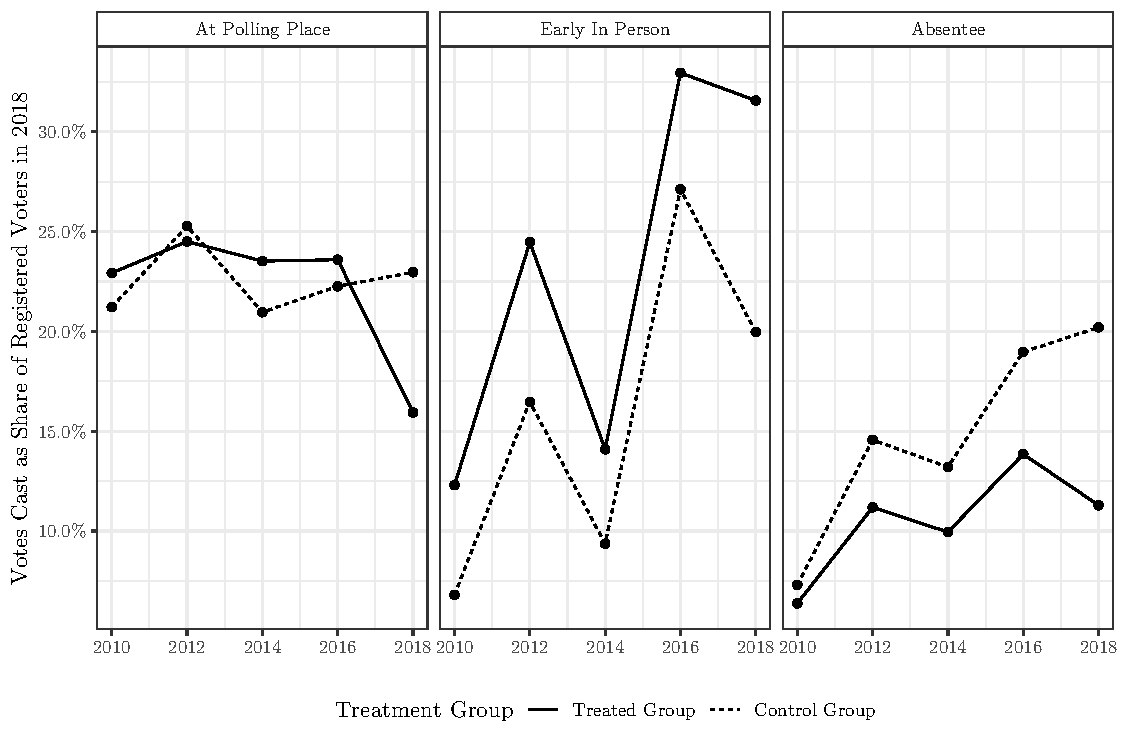
\includegraphics{hurricane_michael_files/figure-latex/vote-mode-chunk-1} 

}

\caption{\label{fig:vote-mode}Share of Voters Participating by Vote Method, 2010 -- 2018}\label{fig:vote-mode-chunk}
\end{figure}

Figure \ref{fig:vote-mode} makes clear that the decline in turnout was a product of lower turnout on election day, and via absentee voting. In fact, turnout among early voters appears to have been \emph{higher} in 2018 than would have been expected based on past behavior and the control voters' participation method in 2018.

The decrease in participation via absentee ballots prompts a follow-up question: the executive order should have made it far easier to vote absentee. Why, then, did a much lower share of voters vote using this method?

To understand why this is the case, we turn to data from the Election Assistance Commission's Election Administration and Voting Survey (EAVS). The EAVS asks election administrators a host of questions after each federal election --- including, importantly, the number of absentee ballots requested. We specifically use EAVS from 2016 and 2018 to understand the changes in the number of absentee ballots requested. In Figure \ref{fig:eavs} we plot the change in the percentage of registered voters who requested an absentee ballot in the two years for each county in Florida. In Palm Beach County, for instance, 19.6 percent of registered voters requested an absentee ballot in 2016, while 23.0 percent did so in 2018. The difference for Palm Beach County in Figure \ref{fig:eavs} is therefore 3.5 percentage points.\footnote{This is not 3.4 percentage points due to rounding.}

\begin{figure}[H]

{\centering 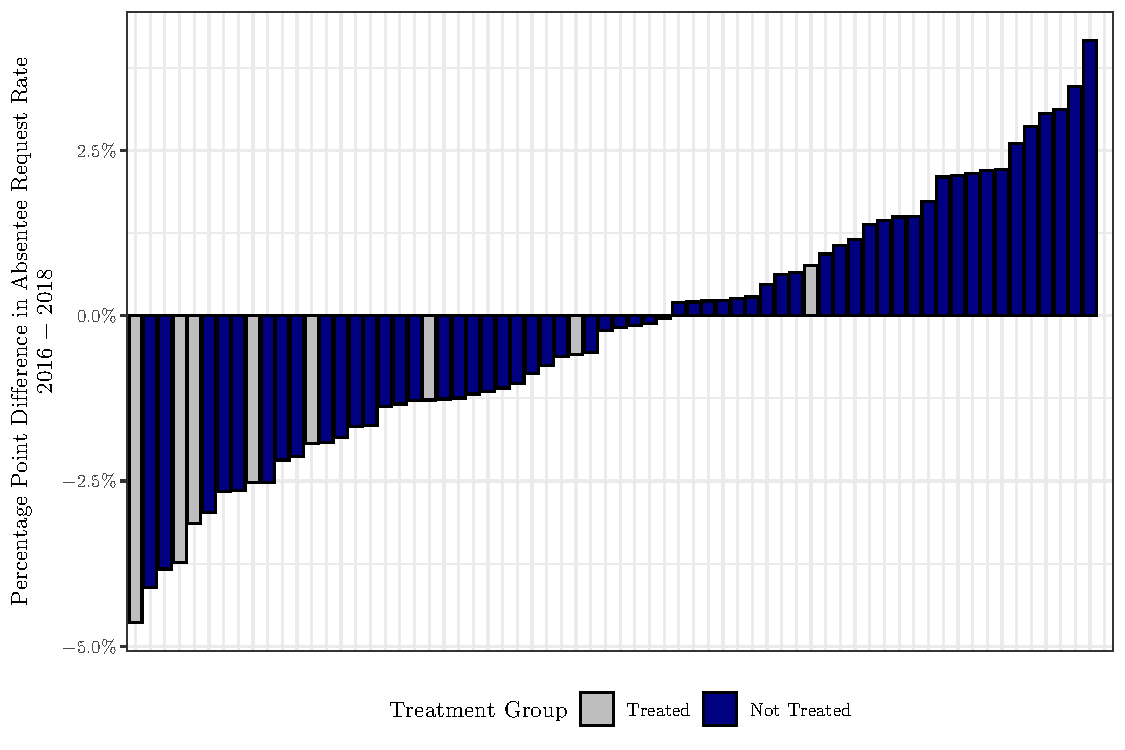
\includegraphics{hurricane_michael_files/figure-latex/eavs-chunk-1} 

}

\caption{\label{fig:eavs}Change in Absentee Ballot Request Rate, 2016 -- 2018}\label{fig:eavs-chunk}
\end{figure}

Sixty-six counties in Florida reported their absentee request rate in both 2016 and 2018. Of the ten counties where the request rate declined by the most, four were treated by the executive order. There were 29 counties where the share of registered voters who requested an absentee ballot increased between 2016 and 2018; just one of the treated counties, however, saw an increase. It appears that Hurricane Michael led to a substantial decrease in the request of absentee ballots. This is despite the fact that Executive Order 18-283 reduced the administrative hurdles to sending ballots to addresses other than the one listed on the voter rolls. It appears that the loosened restrictions were not well communicated to voters throughout the treated counties.

\newpage

\hypertarget{references}{%
\section*{References}\label{references}}
\addcontentsline{toc}{section}{References}

\hypertarget{refs}{}
\begin{cslreferences}
\leavevmode\hypertarget{ref-Abadie2019}{}%
Abadie, Alberto, and Jann Spiess. 2019. ``Robust Post-Matching Inference.'' \emph{Working Paper.}

\leavevmode\hypertarget{ref-Parks2018}{}%
Parks, Miles. 2018. ``After Hurricane Michael, Voting 'Is the Last Thing on Their Minds'.'' \emph{NPR.org}, October 25, 2018. \url{https://www.npr.org/2018/10/25/659819848/after-hurricane-michael-voting-is-the-last-thing-on-their-minds}.

\leavevmode\hypertarget{ref-Sekhon2011}{}%
Sekhon, Jasjeet S. 2011. ``Multivariate and Propensity Score Matching Software with Automated Balance Optimization: The Matching Package for R.'' \emph{Journal of Statistical Software} 42 (1): 1--52. \url{https://doi.org/10.18637/jss.v042.i07}.
\end{cslreferences}

\end{document}
